\hypertarget{_lgm___octree_8h}{
\section{/home/mgh/LanlGeoMag/libLanlGeoMag/Lgm/Lgm\_\-Octree.h File Reference}
\label{_lgm___octree_8h}\index{/home/mgh/LanlGeoMag/libLanlGeoMag/Lgm/Lgm\_\-Octree.h@{/home/mgh/LanlGeoMag/libLanlGeoMag/Lgm/Lgm\_\-Octree.h}}
}
{\tt \#include \char`\"{}Lgm\_\-Vec.h\char`\"{}}\par


Include dependency graph for Lgm\_\-Octree.h:\nopagebreak
\begin{figure}[H]
\begin{center}
\leavevmode
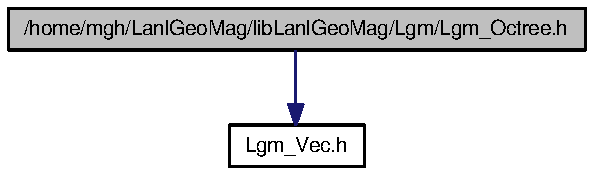
\includegraphics[width=160pt]{_lgm___octree_8h__incl}
\end{center}
\end{figure}


This graph shows which files directly or indirectly include this file:\nopagebreak
\begin{figure}[H]
\begin{center}
\leavevmode

\includegraphics[width=420pt]{_lgm___octree_8h__dep__incl}
\end{center}
\end{figure}
\subsection*{Data Structures}
\begin{CompactItemize}
\item 
struct \hyperlink{struct___lgm___octree_data}{\_\-Lgm\_\-OctreeData}
\item 
struct \hyperlink{struct___lgm___octree_cell}{\_\-Lgm\_\-OctreeCell}
\item 
struct \hyperlink{struct__p_queue}{\_\-pQueue}
\end{CompactItemize}
\subsection*{Defines}
\begin{CompactItemize}
\item 
\#define \hyperlink{_lgm___octree_8h_83d4bc3d9d18688b2119ca2e77c5904c}{OCTREE\_\-MAX\_\-LEVELS}~16
\item 
\#define \hyperlink{_lgm___octree_8h_50cc89ad030d4d45cf6450bf67ab1a6a}{OCTREE\_\-ROOT\_\-LEVEL}~15
\item 
\#define \hyperlink{_lgm___octree_8h_840a13e4ac67b3dece56d79c7ff99b59}{OCTREE\_\-MAX\_\-VAL}~(32768.0)
\item 
\#define \hyperlink{_lgm___octree_8h_4a40a403f3149048e731aa2c41fcf848}{OCTREE\_\-MAX\_\-DATA\_\-PER\_\-OCTANT}~10
\item 
\#define \hyperlink{_lgm___octree_8h_a8cecfc5c5c054d2875c03e77b7be15d}{TRUE}~1
\item 
\#define \hyperlink{_lgm___octree_8h_a93f0eb578d23995850d61f7d61c55c1}{FALSE}~0
\item 
\#define \hyperlink{_lgm___octree_8h_9f3b435ad7cc9c098b3de5d62950a1ca}{OCTREE\_\-KNN\_\-SUCCESS}~1
\item 
\#define \hyperlink{_lgm___octree_8h_b5ea4768ba7862b8601a3ef27d6843f0}{OCTREE\_\-KNN\_\-TOO\_\-FEW\_\-NNS}~0
\item 
\#define \hyperlink{_lgm___octree_8h_2a18af7173f980bc48f9184d3258b502}{OCTREE\_\-KNN\_\-NOT\_\-ENOUGH\_\-DATA}~-1
\item 
\#define \hyperlink{_lgm___octree_8h_72a1f207d0b0d8875f6d549b7b869bfa}{OCTREE\_\-IS\_\-NULL}~-2
\end{CompactItemize}
\subsection*{Typedefs}
\begin{CompactItemize}
\item 
typedef struct \hyperlink{struct___lgm___octree_data}{\_\-Lgm\_\-OctreeData} \hyperlink{_lgm___octree_8h_9425b40ec083efb95518831f6eb142a4}{Lgm\_\-OctreeData}
\item 
typedef struct \hyperlink{struct___lgm___octree_cell}{\_\-Lgm\_\-OctreeCell} \hyperlink{_lgm___octree_8h_d3896773c53b251b3b063cf642c2b290}{Lgm\_\-OctreeCell}
\item 
typedef struct \hyperlink{struct__p_queue}{\_\-pQueue} \hyperlink{_lgm___octree_8h_bdb1526d8d1ed9e1f9c95c582f46a884}{pQueue}
\end{CompactItemize}
\subsection*{Functions}
\begin{CompactItemize}
\item 
void \hyperlink{_lgm___octree_8h_5be6ddcd43586ee6989697d995319c31}{Binary} (unsigned int n, char $\ast$Str)
\item 
void \hyperlink{_lgm___octree_8h_ebbdef4a1addf536593f776187402c39}{Lgm\_\-OctreeFreeBranch} (\hyperlink{struct___lgm___octree_cell}{Lgm\_\-OctreeCell} $\ast$Cell)
\item 
void \hyperlink{_lgm___octree_8h_8966fb8ec73aa1c0e437604568685d13}{Lgm\_\-FreeOctree} (\hyperlink{struct___lgm___octree_cell}{Lgm\_\-OctreeCell} $\ast$ot)
\item 
\hyperlink{struct___lgm___octree_cell}{Lgm\_\-OctreeCell} $\ast$ \hyperlink{_lgm___octree_8h_cf7917181ce8b3f4ceb3f8f6af804889}{Lgm\_\-CreateOctreeRoot} ()
\item 
\hyperlink{struct___lgm___octree_cell}{Lgm\_\-OctreeCell} $\ast$ \hyperlink{_lgm___octree_8h_9b05a3600cfb54efc5f722928e1db5d4}{Lgm\_\-OctreeTraverseToLocCode} (\hyperlink{struct___lgm___octree_cell}{Lgm\_\-OctreeCell} $\ast$Cell, unsigned int ChildLevel, unsigned int xLocationCode, unsigned int yLocationCode, unsigned int zLocationCode)
\item 
\hyperlink{struct___lgm___octree_cell}{Lgm\_\-OctreeCell} $\ast$ \hyperlink{_lgm___octree_8h_271dd512841a7b4308c59db95853b8e1}{Lgm\_\-LocateNearestCell} (\hyperlink{struct___lgm___octree_cell}{Lgm\_\-OctreeCell} $\ast$Root, \hyperlink{struct_lgm___vector}{Lgm\_\-Vector} $\ast$q)
\item 
double \hyperlink{_lgm___octree_8h_07152ce3d1254cca2f4f2d4735de34b7}{MinDist} (\hyperlink{struct___lgm___octree_cell}{Lgm\_\-OctreeCell} $\ast$Cell, \hyperlink{struct_lgm___vector}{Lgm\_\-Vector} $\ast$q)
\item 
double \hyperlink{_lgm___octree_8h_cb735b055954d17d224db5a55dbd14e6}{InsertCell} (\hyperlink{struct___lgm___octree_cell}{Lgm\_\-OctreeCell} $\ast$Cell, \hyperlink{struct_lgm___vector}{Lgm\_\-Vector} $\ast$q, \hyperlink{struct__p_queue}{pQueue} $\ast$$\ast$PQ, double MaxDist2)
\item 
void \hyperlink{_lgm___octree_8h_0128a077b1023c02e79cfaf65a4e6cfc}{InsertPoint} (\hyperlink{struct___lgm___octree_cell}{Lgm\_\-OctreeCell} $\ast$Cell, int j, \hyperlink{struct_lgm___vector}{Lgm\_\-Vector} $\ast$q, \hyperlink{struct__p_queue}{pQueue} $\ast$$\ast$PQ)
\item 
\hyperlink{struct___lgm___octree_cell}{Lgm\_\-OctreeCell} $\ast$ \hyperlink{_lgm___octree_8h_9ff86b033bf330695e810d00ac8022e1}{DescendTowardClosestLeaf} (\hyperlink{struct___lgm___octree_cell}{Lgm\_\-OctreeCell} $\ast$Node, \hyperlink{struct__p_queue}{pQueue} $\ast$$\ast$PQ, \hyperlink{struct_lgm___vector}{Lgm\_\-Vector} $\ast$q, double MaxDist2)
\item 
\hyperlink{struct__p_queue}{pQueue} $\ast$ \hyperlink{_lgm___octree_8h_653f08b2912abb5a5fb6c1761b8a8cec}{PopObj} (\hyperlink{struct__p_queue}{pQueue} $\ast$$\ast$PQ)
\item 
int \hyperlink{_lgm___octree_8h_885f0695706ada1ee750180afe105958}{Lgm\_\-Octree\_\-kNN} (\hyperlink{struct_lgm___vector}{Lgm\_\-Vector} $\ast$q, \hyperlink{struct___lgm___octree_cell}{Lgm\_\-OctreeCell} $\ast$Root, int K, int $\ast$Kgot, double MaxDist2, \hyperlink{struct___lgm___octree_data}{Lgm\_\-OctreeData} $\ast$kNN)
\item 
\hyperlink{struct___lgm___octree_cell}{Lgm\_\-OctreeCell} $\ast$ \hyperlink{_lgm___octree_8h_8faba8ef3514ee1be8aedd369afd4db9}{CreateNewOctants} (\hyperlink{struct___lgm___octree_cell}{Lgm\_\-OctreeCell} $\ast$Parent)
\item 
void \hyperlink{_lgm___octree_8h_3df40f5467250c1b9c2ba1053d38d76f}{SubDivideVolume} (\hyperlink{struct___lgm___octree_cell}{Lgm\_\-OctreeCell} $\ast$Vol)
\item 
\hyperlink{struct___lgm___octree_cell}{Lgm\_\-OctreeCell} $\ast$ \hyperlink{_lgm___octree_8h_20080c6b6bf182550e7c1e99d3807020}{Lgm\_\-InitOctree} (\hyperlink{struct_lgm___vector}{Lgm\_\-Vector} $\ast$ObjectPoints, \hyperlink{struct_lgm___vector}{Lgm\_\-Vector} $\ast$ObjectData, unsigned long int N, double $\ast$Min, double $\ast$Max, double $\ast$Diff)
\end{CompactItemize}


\subsection{Define Documentation}
\hypertarget{_lgm___octree_8h_83d4bc3d9d18688b2119ca2e77c5904c}{
\index{Lgm\_\-Octree.h@{Lgm\_\-Octree.h}!OCTREE\_\-MAX\_\-LEVELS@{OCTREE\_\-MAX\_\-LEVELS}}
\index{OCTREE\_\-MAX\_\-LEVELS@{OCTREE\_\-MAX\_\-LEVELS}!Lgm_Octree.h@{Lgm\_\-Octree.h}}
\subsubsection[{OCTREE\_\-MAX\_\-LEVELS}]{\setlength{\rightskip}{0pt plus 5cm}\#define OCTREE\_\-MAX\_\-LEVELS~16}}
\label{_lgm___octree_8h_83d4bc3d9d18688b2119ca2e77c5904c}




Definition at line 6 of file Lgm\_\-Octree.h.\hypertarget{_lgm___octree_8h_50cc89ad030d4d45cf6450bf67ab1a6a}{
\index{Lgm\_\-Octree.h@{Lgm\_\-Octree.h}!OCTREE\_\-ROOT\_\-LEVEL@{OCTREE\_\-ROOT\_\-LEVEL}}
\index{OCTREE\_\-ROOT\_\-LEVEL@{OCTREE\_\-ROOT\_\-LEVEL}!Lgm_Octree.h@{Lgm\_\-Octree.h}}
\subsubsection[{OCTREE\_\-ROOT\_\-LEVEL}]{\setlength{\rightskip}{0pt plus 5cm}\#define OCTREE\_\-ROOT\_\-LEVEL~15}}
\label{_lgm___octree_8h_50cc89ad030d4d45cf6450bf67ab1a6a}




Definition at line 7 of file Lgm\_\-Octree.h.\hypertarget{_lgm___octree_8h_840a13e4ac67b3dece56d79c7ff99b59}{
\index{Lgm\_\-Octree.h@{Lgm\_\-Octree.h}!OCTREE\_\-MAX\_\-VAL@{OCTREE\_\-MAX\_\-VAL}}
\index{OCTREE\_\-MAX\_\-VAL@{OCTREE\_\-MAX\_\-VAL}!Lgm_Octree.h@{Lgm\_\-Octree.h}}
\subsubsection[{OCTREE\_\-MAX\_\-VAL}]{\setlength{\rightskip}{0pt plus 5cm}\#define OCTREE\_\-MAX\_\-VAL~(32768.0)}}
\label{_lgm___octree_8h_840a13e4ac67b3dece56d79c7ff99b59}




Definition at line 8 of file Lgm\_\-Octree.h.\hypertarget{_lgm___octree_8h_4a40a403f3149048e731aa2c41fcf848}{
\index{Lgm\_\-Octree.h@{Lgm\_\-Octree.h}!OCTREE\_\-MAX\_\-DATA\_\-PER\_\-OCTANT@{OCTREE\_\-MAX\_\-DATA\_\-PER\_\-OCTANT}}
\index{OCTREE\_\-MAX\_\-DATA\_\-PER\_\-OCTANT@{OCTREE\_\-MAX\_\-DATA\_\-PER\_\-OCTANT}!Lgm_Octree.h@{Lgm\_\-Octree.h}}
\subsubsection[{OCTREE\_\-MAX\_\-DATA\_\-PER\_\-OCTANT}]{\setlength{\rightskip}{0pt plus 5cm}\#define OCTREE\_\-MAX\_\-DATA\_\-PER\_\-OCTANT~10}}
\label{_lgm___octree_8h_4a40a403f3149048e731aa2c41fcf848}




Definition at line 9 of file Lgm\_\-Octree.h.\hypertarget{_lgm___octree_8h_a8cecfc5c5c054d2875c03e77b7be15d}{
\index{Lgm\_\-Octree.h@{Lgm\_\-Octree.h}!TRUE@{TRUE}}
\index{TRUE@{TRUE}!Lgm_Octree.h@{Lgm\_\-Octree.h}}
\subsubsection[{TRUE}]{\setlength{\rightskip}{0pt plus 5cm}\#define TRUE~1}}
\label{_lgm___octree_8h_a8cecfc5c5c054d2875c03e77b7be15d}




Definition at line 11 of file Lgm\_\-Octree.h.\hypertarget{_lgm___octree_8h_a93f0eb578d23995850d61f7d61c55c1}{
\index{Lgm\_\-Octree.h@{Lgm\_\-Octree.h}!FALSE@{FALSE}}
\index{FALSE@{FALSE}!Lgm_Octree.h@{Lgm\_\-Octree.h}}
\subsubsection[{FALSE}]{\setlength{\rightskip}{0pt plus 5cm}\#define FALSE~0}}
\label{_lgm___octree_8h_a93f0eb578d23995850d61f7d61c55c1}




Definition at line 12 of file Lgm\_\-Octree.h.\hypertarget{_lgm___octree_8h_9f3b435ad7cc9c098b3de5d62950a1ca}{
\index{Lgm\_\-Octree.h@{Lgm\_\-Octree.h}!OCTREE\_\-KNN\_\-SUCCESS@{OCTREE\_\-KNN\_\-SUCCESS}}
\index{OCTREE\_\-KNN\_\-SUCCESS@{OCTREE\_\-KNN\_\-SUCCESS}!Lgm_Octree.h@{Lgm\_\-Octree.h}}
\subsubsection[{OCTREE\_\-KNN\_\-SUCCESS}]{\setlength{\rightskip}{0pt plus 5cm}\#define OCTREE\_\-KNN\_\-SUCCESS~1}}
\label{_lgm___octree_8h_9f3b435ad7cc9c098b3de5d62950a1ca}




Definition at line 15 of file Lgm\_\-Octree.h.\hypertarget{_lgm___octree_8h_b5ea4768ba7862b8601a3ef27d6843f0}{
\index{Lgm\_\-Octree.h@{Lgm\_\-Octree.h}!OCTREE\_\-KNN\_\-TOO\_\-FEW\_\-NNS@{OCTREE\_\-KNN\_\-TOO\_\-FEW\_\-NNS}}
\index{OCTREE\_\-KNN\_\-TOO\_\-FEW\_\-NNS@{OCTREE\_\-KNN\_\-TOO\_\-FEW\_\-NNS}!Lgm_Octree.h@{Lgm\_\-Octree.h}}
\subsubsection[{OCTREE\_\-KNN\_\-TOO\_\-FEW\_\-NNS}]{\setlength{\rightskip}{0pt plus 5cm}\#define OCTREE\_\-KNN\_\-TOO\_\-FEW\_\-NNS~0}}
\label{_lgm___octree_8h_b5ea4768ba7862b8601a3ef27d6843f0}




Definition at line 16 of file Lgm\_\-Octree.h.\hypertarget{_lgm___octree_8h_2a18af7173f980bc48f9184d3258b502}{
\index{Lgm\_\-Octree.h@{Lgm\_\-Octree.h}!OCTREE\_\-KNN\_\-NOT\_\-ENOUGH\_\-DATA@{OCTREE\_\-KNN\_\-NOT\_\-ENOUGH\_\-DATA}}
\index{OCTREE\_\-KNN\_\-NOT\_\-ENOUGH\_\-DATA@{OCTREE\_\-KNN\_\-NOT\_\-ENOUGH\_\-DATA}!Lgm_Octree.h@{Lgm\_\-Octree.h}}
\subsubsection[{OCTREE\_\-KNN\_\-NOT\_\-ENOUGH\_\-DATA}]{\setlength{\rightskip}{0pt plus 5cm}\#define OCTREE\_\-KNN\_\-NOT\_\-ENOUGH\_\-DATA~-1}}
\label{_lgm___octree_8h_2a18af7173f980bc48f9184d3258b502}




Definition at line 17 of file Lgm\_\-Octree.h.\hypertarget{_lgm___octree_8h_72a1f207d0b0d8875f6d549b7b869bfa}{
\index{Lgm\_\-Octree.h@{Lgm\_\-Octree.h}!OCTREE\_\-IS\_\-NULL@{OCTREE\_\-IS\_\-NULL}}
\index{OCTREE\_\-IS\_\-NULL@{OCTREE\_\-IS\_\-NULL}!Lgm_Octree.h@{Lgm\_\-Octree.h}}
\subsubsection[{OCTREE\_\-IS\_\-NULL}]{\setlength{\rightskip}{0pt plus 5cm}\#define OCTREE\_\-IS\_\-NULL~-2}}
\label{_lgm___octree_8h_72a1f207d0b0d8875f6d549b7b869bfa}




Definition at line 19 of file Lgm\_\-Octree.h.

\subsection{Typedef Documentation}
\hypertarget{_lgm___octree_8h_9425b40ec083efb95518831f6eb142a4}{
\index{Lgm\_\-Octree.h@{Lgm\_\-Octree.h}!Lgm\_\-OctreeData@{Lgm\_\-OctreeData}}
\index{Lgm\_\-OctreeData@{Lgm\_\-OctreeData}!Lgm_Octree.h@{Lgm\_\-Octree.h}}
\subsubsection[{Lgm\_\-OctreeData}]{\setlength{\rightskip}{0pt plus 5cm}typedef struct {\bf \_\-Lgm\_\-OctreeData}  {\bf Lgm\_\-OctreeData}}}
\label{_lgm___octree_8h_9425b40ec083efb95518831f6eb142a4}


\hypertarget{_lgm___octree_8h_d3896773c53b251b3b063cf642c2b290}{
\index{Lgm\_\-Octree.h@{Lgm\_\-Octree.h}!Lgm\_\-OctreeCell@{Lgm\_\-OctreeCell}}
\index{Lgm\_\-OctreeCell@{Lgm\_\-OctreeCell}!Lgm_Octree.h@{Lgm\_\-Octree.h}}
\subsubsection[{Lgm\_\-OctreeCell}]{\setlength{\rightskip}{0pt plus 5cm}typedef struct {\bf \_\-Lgm\_\-OctreeCell}  {\bf Lgm\_\-OctreeCell}}}
\label{_lgm___octree_8h_d3896773c53b251b3b063cf642c2b290}


\hypertarget{_lgm___octree_8h_bdb1526d8d1ed9e1f9c95c582f46a884}{
\index{Lgm\_\-Octree.h@{Lgm\_\-Octree.h}!pQueue@{pQueue}}
\index{pQueue@{pQueue}!Lgm_Octree.h@{Lgm\_\-Octree.h}}
\subsubsection[{pQueue}]{\setlength{\rightskip}{0pt plus 5cm}typedef struct {\bf \_\-pQueue}  {\bf pQueue}}}
\label{_lgm___octree_8h_bdb1526d8d1ed9e1f9c95c582f46a884}




\subsection{Function Documentation}
\hypertarget{_lgm___octree_8h_5be6ddcd43586ee6989697d995319c31}{
\index{Lgm\_\-Octree.h@{Lgm\_\-Octree.h}!Binary@{Binary}}
\index{Binary@{Binary}!Lgm_Octree.h@{Lgm\_\-Octree.h}}
\subsubsection[{Binary}]{\setlength{\rightskip}{0pt plus 5cm}void Binary (unsigned int {\em n}, \/  char $\ast$ {\em Str})}}
\label{_lgm___octree_8h_5be6ddcd43586ee6989697d995319c31}




Definition at line 13 of file Lgm\_\-Octree.c.\hypertarget{_lgm___octree_8h_ebbdef4a1addf536593f776187402c39}{
\index{Lgm\_\-Octree.h@{Lgm\_\-Octree.h}!Lgm\_\-OctreeFreeBranch@{Lgm\_\-OctreeFreeBranch}}
\index{Lgm\_\-OctreeFreeBranch@{Lgm\_\-OctreeFreeBranch}!Lgm_Octree.h@{Lgm\_\-Octree.h}}
\subsubsection[{Lgm\_\-OctreeFreeBranch}]{\setlength{\rightskip}{0pt plus 5cm}void Lgm\_\-OctreeFreeBranch ({\bf Lgm\_\-OctreeCell} $\ast$ {\em Cell})}}
\label{_lgm___octree_8h_ebbdef4a1addf536593f776187402c39}




Definition at line 30 of file Lgm\_\-Octree.c.

Here is the call graph for this function:\nopagebreak
\begin{figure}[H]
\begin{center}
\leavevmode
\includegraphics[width=82pt]{_lgm___octree_8h_ebbdef4a1addf536593f776187402c39_cgraph}
\end{center}
\end{figure}


Here is the caller graph for this function:\nopagebreak
\begin{figure}[H]
\begin{center}
\leavevmode
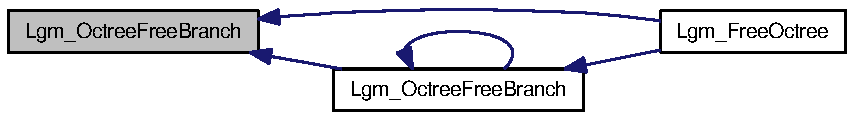
\includegraphics[width=223pt]{_lgm___octree_8h_ebbdef4a1addf536593f776187402c39_icgraph}
\end{center}
\end{figure}
\hypertarget{_lgm___octree_8h_8966fb8ec73aa1c0e437604568685d13}{
\index{Lgm\_\-Octree.h@{Lgm\_\-Octree.h}!Lgm\_\-FreeOctree@{Lgm\_\-FreeOctree}}
\index{Lgm\_\-FreeOctree@{Lgm\_\-FreeOctree}!Lgm_Octree.h@{Lgm\_\-Octree.h}}
\subsubsection[{Lgm\_\-FreeOctree}]{\setlength{\rightskip}{0pt plus 5cm}void Lgm\_\-FreeOctree ({\bf Lgm\_\-OctreeCell} $\ast$ {\em ot})}}
\label{_lgm___octree_8h_8966fb8ec73aa1c0e437604568685d13}




Definition at line 58 of file Lgm\_\-Octree.c.

Here is the call graph for this function:\nopagebreak
\begin{figure}[H]
\begin{center}
\leavevmode
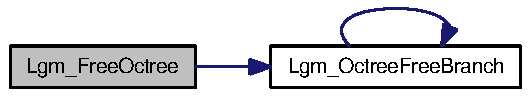
\includegraphics[width=145pt]{_lgm___octree_8h_8966fb8ec73aa1c0e437604568685d13_cgraph}
\end{center}
\end{figure}
\hypertarget{_lgm___octree_8h_cf7917181ce8b3f4ceb3f8f6af804889}{
\index{Lgm\_\-Octree.h@{Lgm\_\-Octree.h}!Lgm\_\-CreateOctreeRoot@{Lgm\_\-CreateOctreeRoot}}
\index{Lgm\_\-CreateOctreeRoot@{Lgm\_\-CreateOctreeRoot}!Lgm_Octree.h@{Lgm\_\-Octree.h}}
\subsubsection[{Lgm\_\-CreateOctreeRoot}]{\setlength{\rightskip}{0pt plus 5cm}{\bf Lgm\_\-OctreeCell}$\ast$ Lgm\_\-CreateOctreeRoot ()}}
\label{_lgm___octree_8h_cf7917181ce8b3f4ceb3f8f6af804889}




Definition at line 64 of file Lgm\_\-Octree.c.

Here is the caller graph for this function:\nopagebreak
\begin{figure}[H]
\begin{center}
\leavevmode
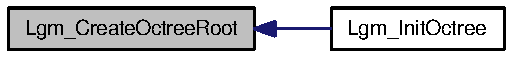
\includegraphics[width=141pt]{_lgm___octree_8h_cf7917181ce8b3f4ceb3f8f6af804889_icgraph}
\end{center}
\end{figure}
\hypertarget{_lgm___octree_8h_9b05a3600cfb54efc5f722928e1db5d4}{
\index{Lgm\_\-Octree.h@{Lgm\_\-Octree.h}!Lgm\_\-OctreeTraverseToLocCode@{Lgm\_\-OctreeTraverseToLocCode}}
\index{Lgm\_\-OctreeTraverseToLocCode@{Lgm\_\-OctreeTraverseToLocCode}!Lgm_Octree.h@{Lgm\_\-Octree.h}}
\subsubsection[{Lgm\_\-OctreeTraverseToLocCode}]{\setlength{\rightskip}{0pt plus 5cm}{\bf Lgm\_\-OctreeCell}$\ast$ Lgm\_\-OctreeTraverseToLocCode ({\bf Lgm\_\-OctreeCell} $\ast$ {\em Cell}, \/  unsigned int {\em ChildLevel}, \/  unsigned int {\em xLocationCode}, \/  unsigned int {\em yLocationCode}, \/  unsigned int {\em zLocationCode})}}
\label{_lgm___octree_8h_9b05a3600cfb54efc5f722928e1db5d4}




Definition at line 99 of file Lgm\_\-Octree.c.

Here is the caller graph for this function:\nopagebreak
\begin{figure}[H]
\begin{center}
\leavevmode
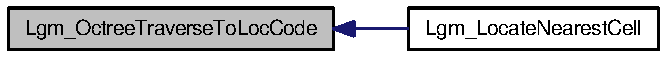
\includegraphics[width=178pt]{_lgm___octree_8h_9b05a3600cfb54efc5f722928e1db5d4_icgraph}
\end{center}
\end{figure}
\hypertarget{_lgm___octree_8h_271dd512841a7b4308c59db95853b8e1}{
\index{Lgm\_\-Octree.h@{Lgm\_\-Octree.h}!Lgm\_\-LocateNearestCell@{Lgm\_\-LocateNearestCell}}
\index{Lgm\_\-LocateNearestCell@{Lgm\_\-LocateNearestCell}!Lgm_Octree.h@{Lgm\_\-Octree.h}}
\subsubsection[{Lgm\_\-LocateNearestCell}]{\setlength{\rightskip}{0pt plus 5cm}{\bf Lgm\_\-OctreeCell}$\ast$ Lgm\_\-LocateNearestCell ({\bf Lgm\_\-OctreeCell} $\ast$ {\em Root}, \/  {\bf Lgm\_\-Vector} $\ast$ {\em q})}}
\label{_lgm___octree_8h_271dd512841a7b4308c59db95853b8e1}




Definition at line 127 of file Lgm\_\-Octree.c.

Here is the call graph for this function:\nopagebreak
\begin{figure}[H]
\begin{center}
\leavevmode
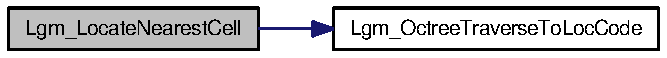
\includegraphics[width=178pt]{_lgm___octree_8h_271dd512841a7b4308c59db95853b8e1_cgraph}
\end{center}
\end{figure}
\hypertarget{_lgm___octree_8h_07152ce3d1254cca2f4f2d4735de34b7}{
\index{Lgm\_\-Octree.h@{Lgm\_\-Octree.h}!MinDist@{MinDist}}
\index{MinDist@{MinDist}!Lgm_Octree.h@{Lgm\_\-Octree.h}}
\subsubsection[{MinDist}]{\setlength{\rightskip}{0pt plus 5cm}double MinDist ({\bf Lgm\_\-OctreeCell} $\ast$ {\em Cell}, \/  {\bf Lgm\_\-Vector} $\ast$ {\em q})}}
\label{_lgm___octree_8h_07152ce3d1254cca2f4f2d4735de34b7}




Definition at line 162 of file Lgm\_\-Octree.c.

Here is the caller graph for this function:\nopagebreak
\begin{figure}[H]
\begin{center}
\leavevmode
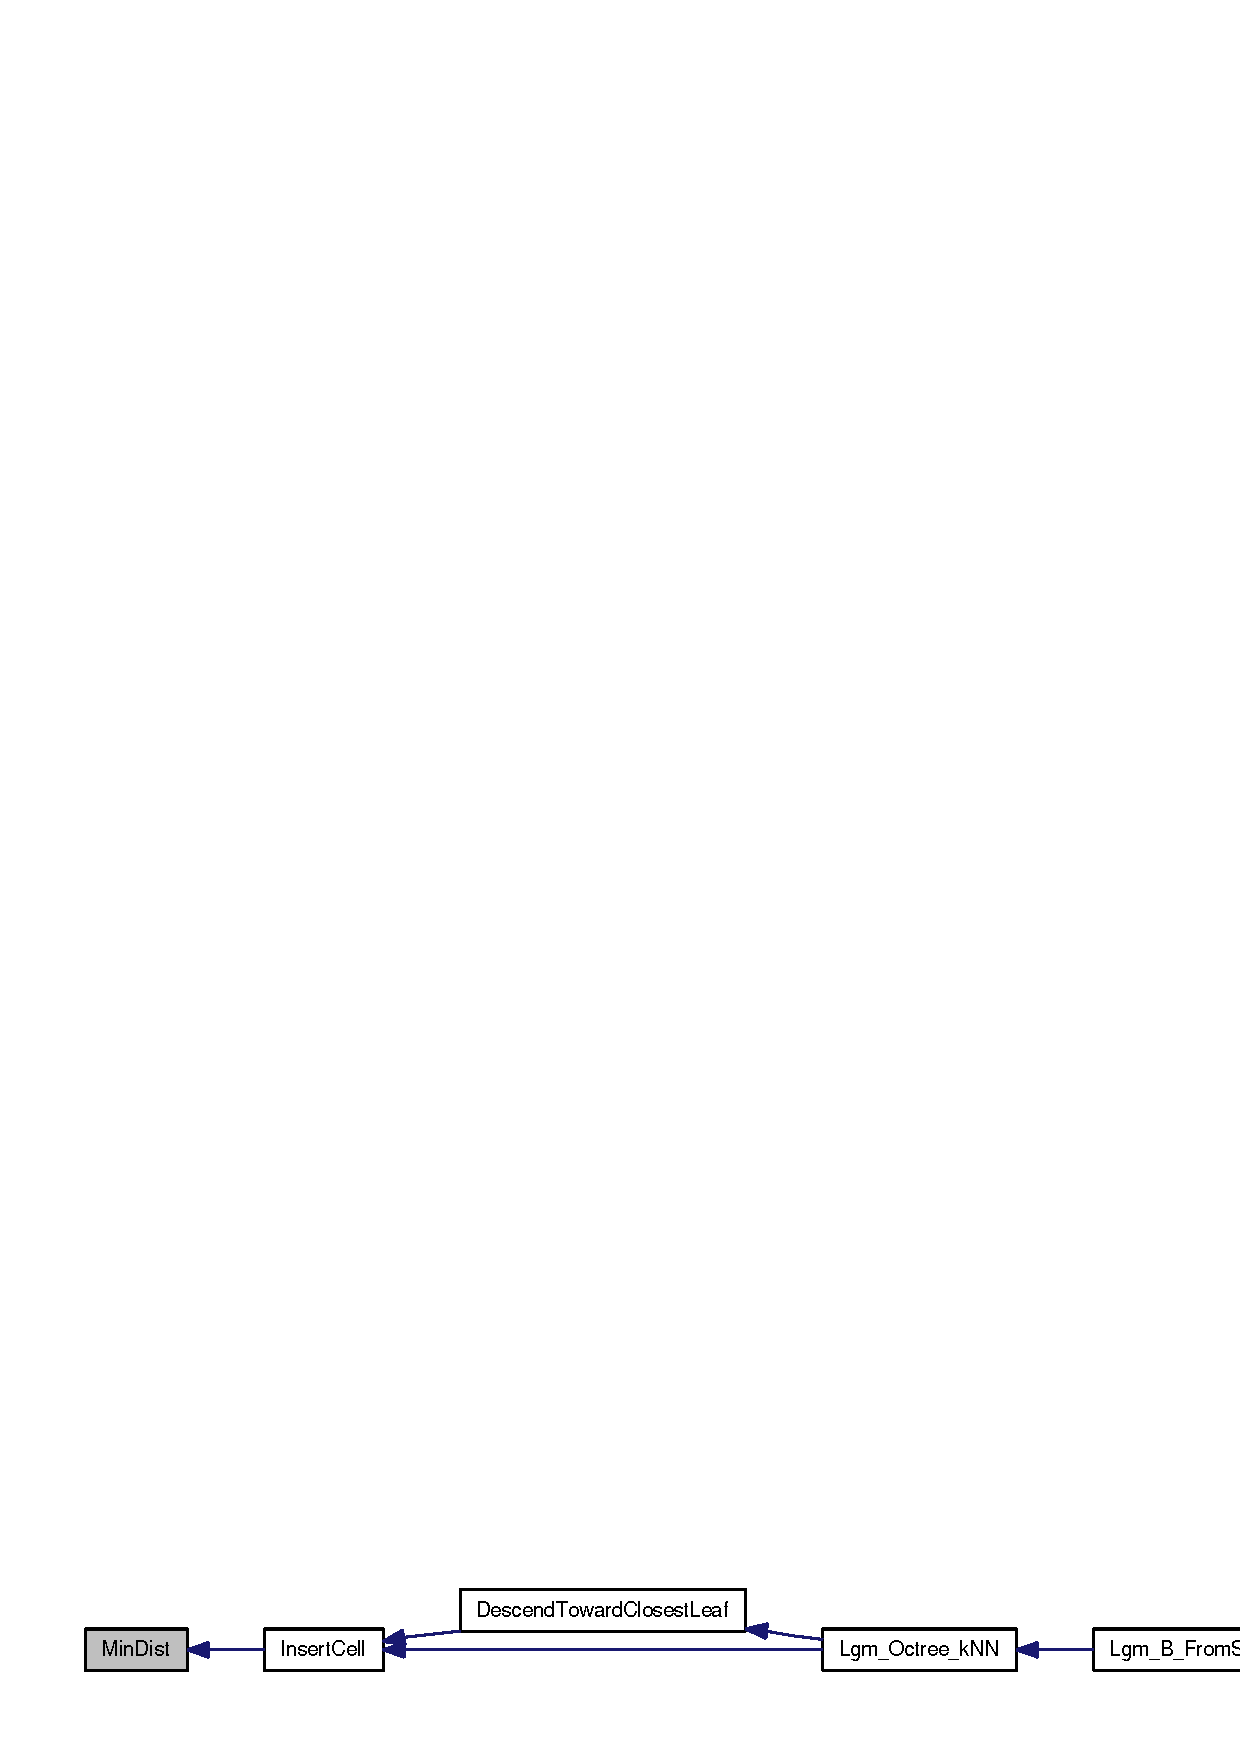
\includegraphics[width=333pt]{_lgm___octree_8h_07152ce3d1254cca2f4f2d4735de34b7_icgraph}
\end{center}
\end{figure}
\hypertarget{_lgm___octree_8h_cb735b055954d17d224db5a55dbd14e6}{
\index{Lgm\_\-Octree.h@{Lgm\_\-Octree.h}!InsertCell@{InsertCell}}
\index{InsertCell@{InsertCell}!Lgm_Octree.h@{Lgm\_\-Octree.h}}
\subsubsection[{InsertCell}]{\setlength{\rightskip}{0pt plus 5cm}double InsertCell ({\bf Lgm\_\-OctreeCell} $\ast$ {\em Cell}, \/  {\bf Lgm\_\-Vector} $\ast$ {\em q}, \/  {\bf pQueue} $\ast$$\ast$ {\em PQ}, \/  double {\em MaxDist2})}}
\label{_lgm___octree_8h_cb735b055954d17d224db5a55dbd14e6}




Definition at line 198 of file Lgm\_\-Octree.c.

Here is the call graph for this function:\nopagebreak
\begin{figure}[H]
\begin{center}
\leavevmode
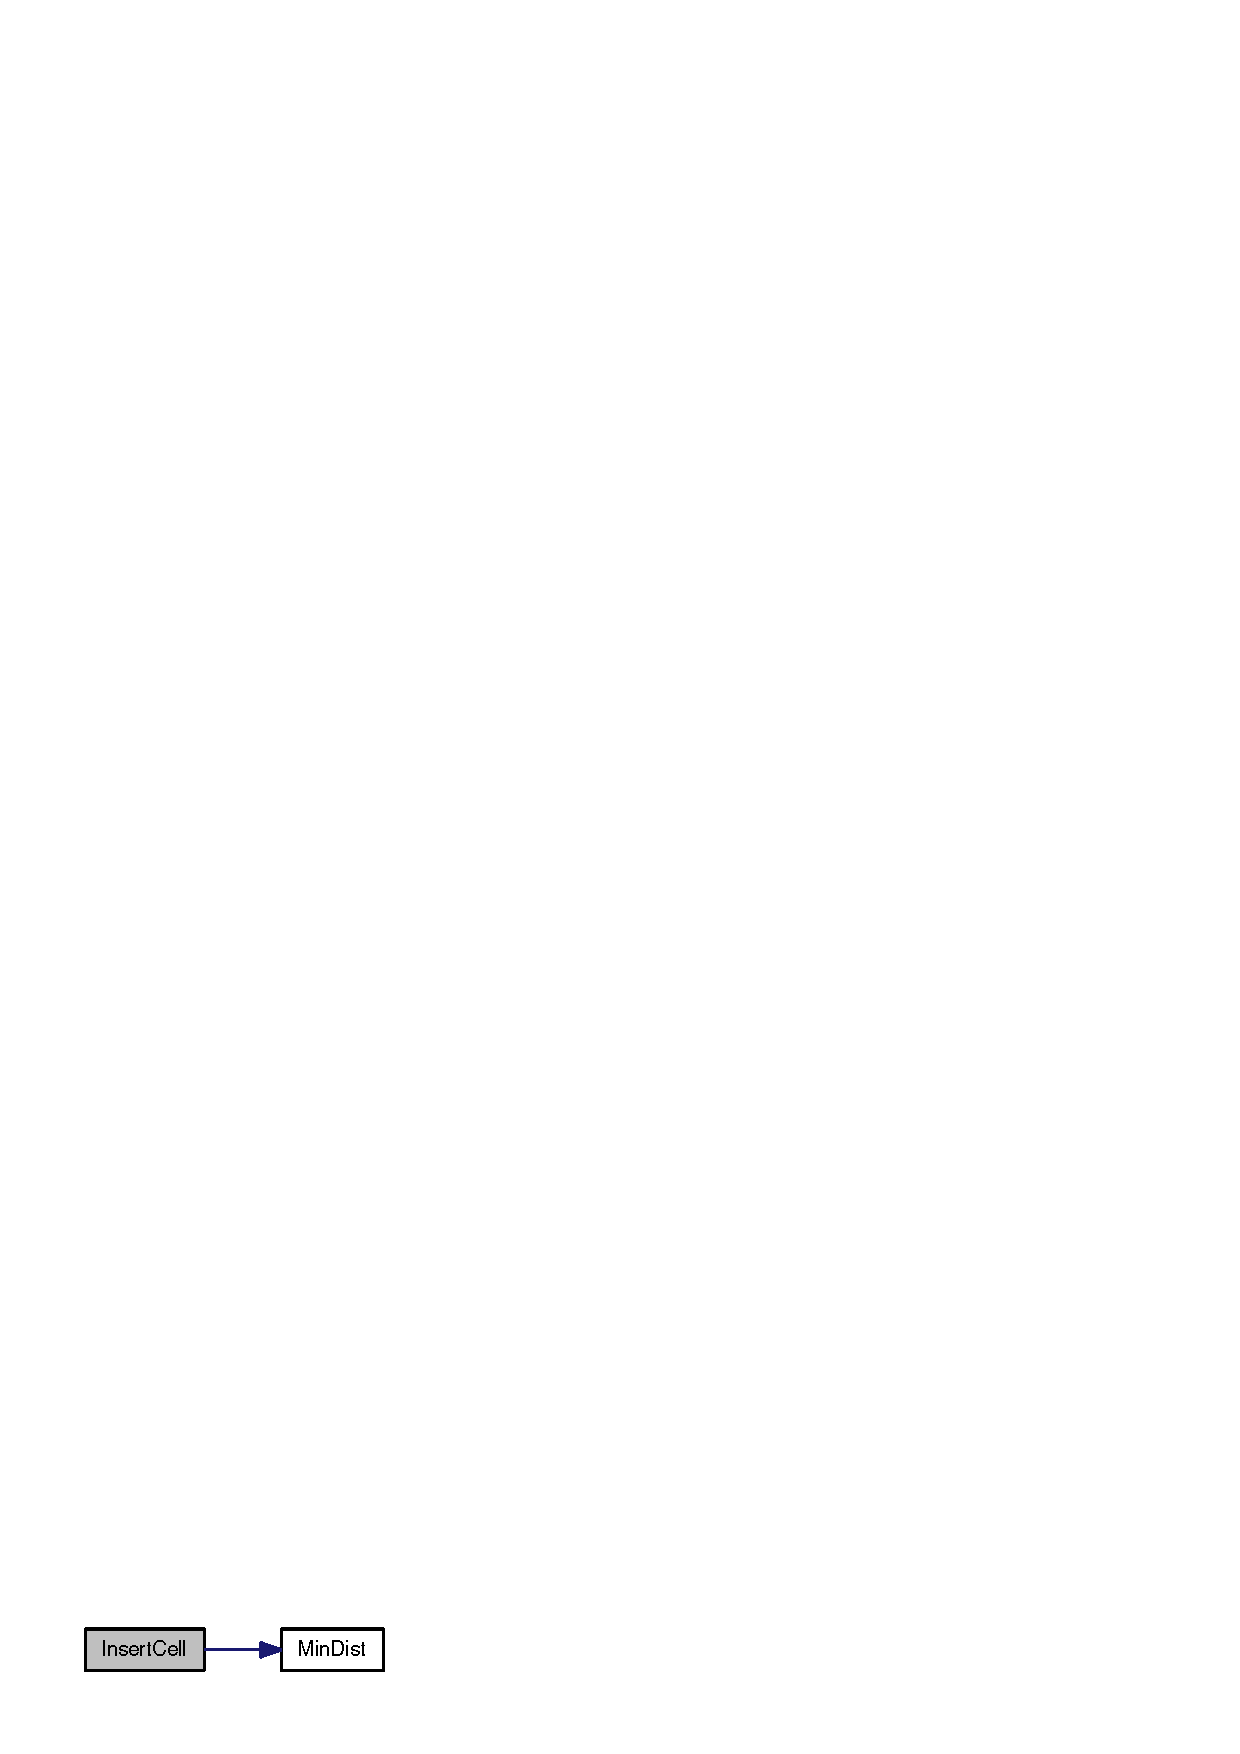
\includegraphics[width=94pt]{_lgm___octree_8h_cb735b055954d17d224db5a55dbd14e6_cgraph}
\end{center}
\end{figure}


Here is the caller graph for this function:\nopagebreak
\begin{figure}[H]
\begin{center}
\leavevmode
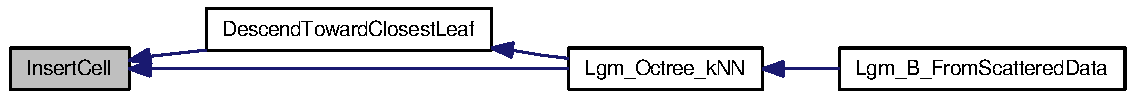
\includegraphics[width=290pt]{_lgm___octree_8h_cb735b055954d17d224db5a55dbd14e6_icgraph}
\end{center}
\end{figure}
\hypertarget{_lgm___octree_8h_0128a077b1023c02e79cfaf65a4e6cfc}{
\index{Lgm\_\-Octree.h@{Lgm\_\-Octree.h}!InsertPoint@{InsertPoint}}
\index{InsertPoint@{InsertPoint}!Lgm_Octree.h@{Lgm\_\-Octree.h}}
\subsubsection[{InsertPoint}]{\setlength{\rightskip}{0pt plus 5cm}void InsertPoint ({\bf Lgm\_\-OctreeCell} $\ast$ {\em Cell}, \/  int {\em j}, \/  {\bf Lgm\_\-Vector} $\ast$ {\em q}, \/  {\bf pQueue} $\ast$$\ast$ {\em PQ})}}
\label{_lgm___octree_8h_0128a077b1023c02e79cfaf65a4e6cfc}




Definition at line 282 of file Lgm\_\-Octree.c.

Here is the caller graph for this function:\nopagebreak
\begin{figure}[H]
\begin{center}
\leavevmode
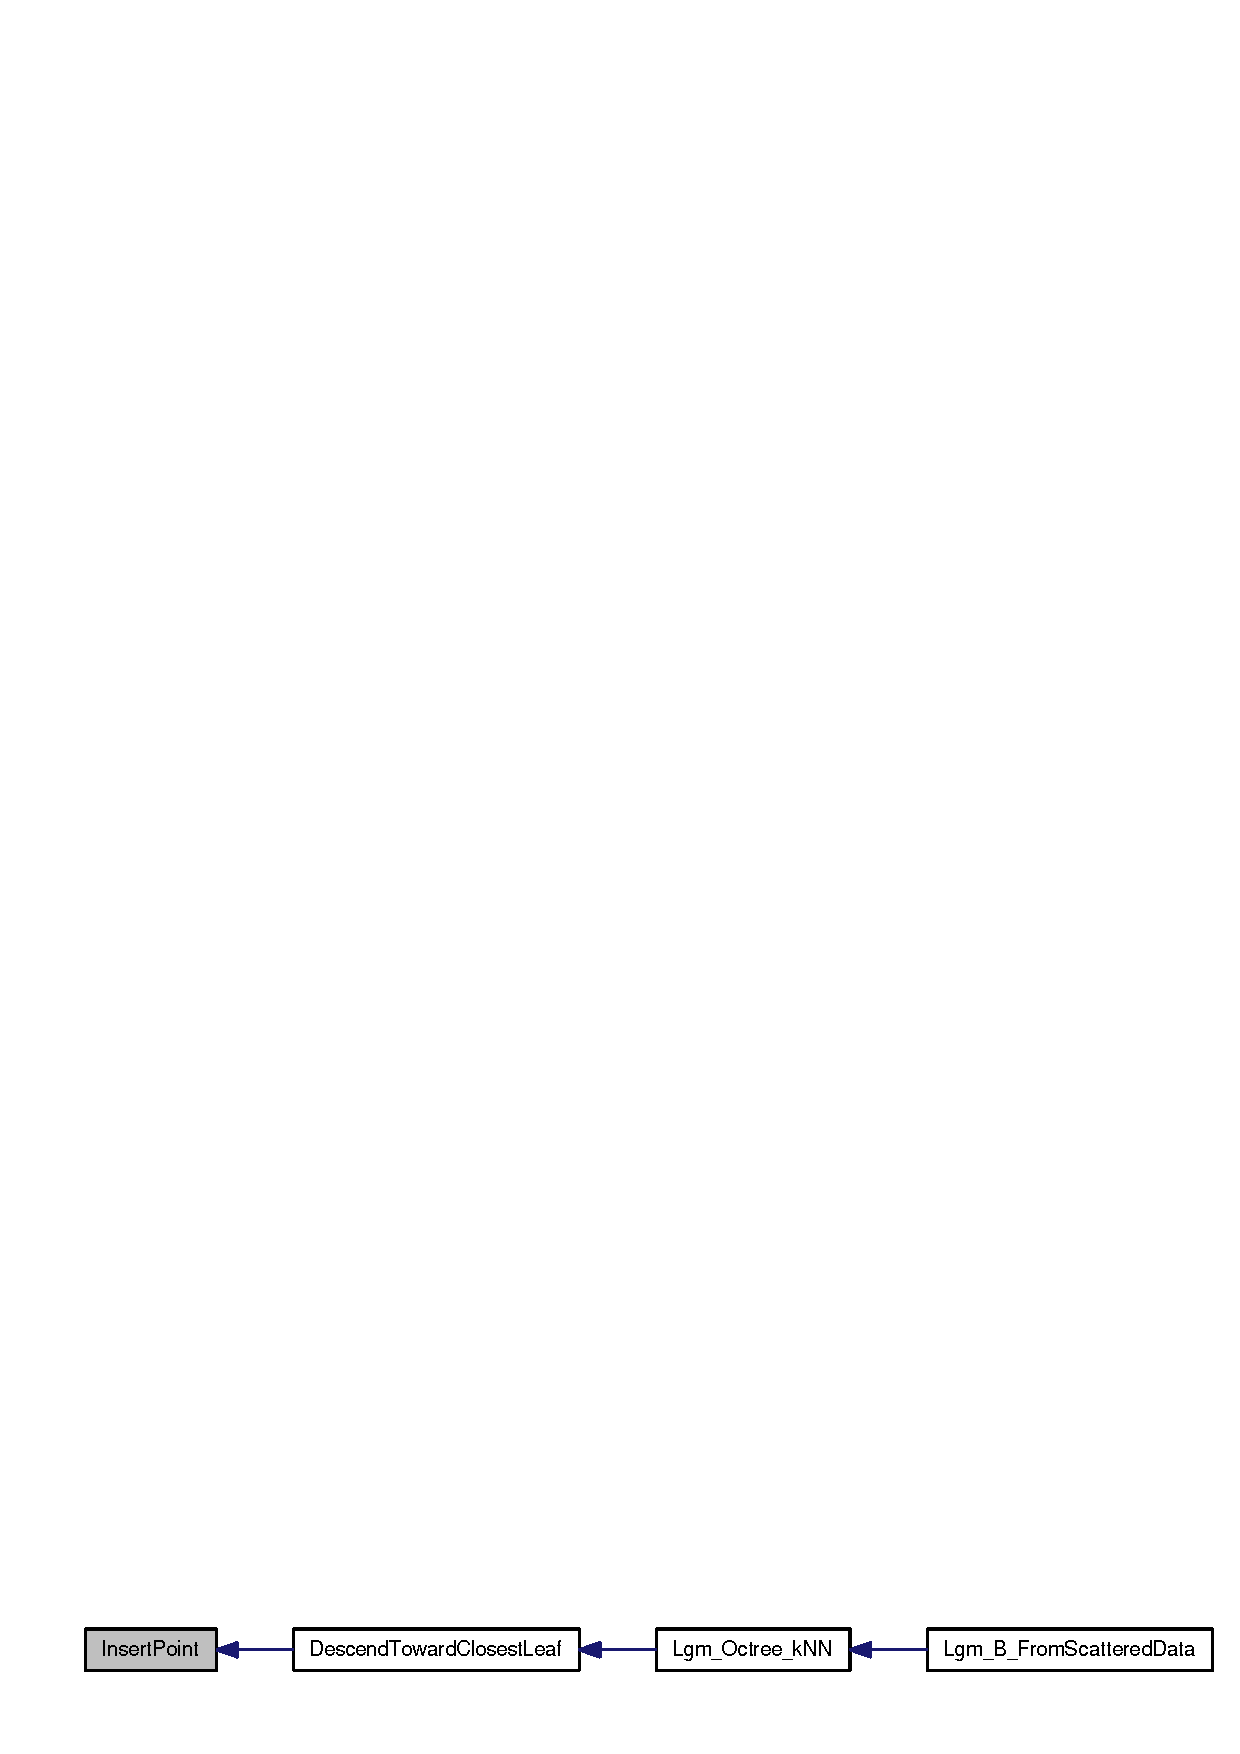
\includegraphics[width=293pt]{_lgm___octree_8h_0128a077b1023c02e79cfaf65a4e6cfc_icgraph}
\end{center}
\end{figure}
\hypertarget{_lgm___octree_8h_9ff86b033bf330695e810d00ac8022e1}{
\index{Lgm\_\-Octree.h@{Lgm\_\-Octree.h}!DescendTowardClosestLeaf@{DescendTowardClosestLeaf}}
\index{DescendTowardClosestLeaf@{DescendTowardClosestLeaf}!Lgm_Octree.h@{Lgm\_\-Octree.h}}
\subsubsection[{DescendTowardClosestLeaf}]{\setlength{\rightskip}{0pt plus 5cm}{\bf Lgm\_\-OctreeCell}$\ast$ DescendTowardClosestLeaf ({\bf Lgm\_\-OctreeCell} $\ast$ {\em Node}, \/  {\bf pQueue} $\ast$$\ast$ {\em PQ}, \/  {\bf Lgm\_\-Vector} $\ast$ {\em q}, \/  double {\em MaxDist2})}}
\label{_lgm___octree_8h_9ff86b033bf330695e810d00ac8022e1}




Definition at line 350 of file Lgm\_\-Octree.c.

Here is the call graph for this function:\nopagebreak
\begin{figure}[H]
\begin{center}
\leavevmode
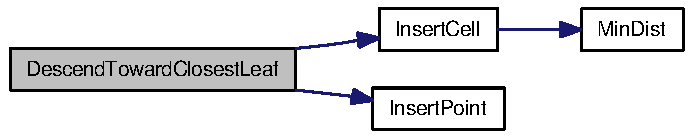
\includegraphics[width=184pt]{_lgm___octree_8h_9ff86b033bf330695e810d00ac8022e1_cgraph}
\end{center}
\end{figure}


Here is the caller graph for this function:\nopagebreak
\begin{figure}[H]
\begin{center}
\leavevmode
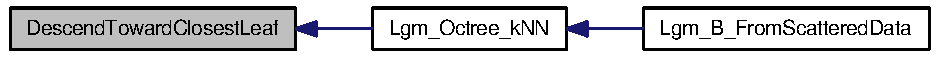
\includegraphics[width=243pt]{_lgm___octree_8h_9ff86b033bf330695e810d00ac8022e1_icgraph}
\end{center}
\end{figure}
\hypertarget{_lgm___octree_8h_653f08b2912abb5a5fb6c1761b8a8cec}{
\index{Lgm\_\-Octree.h@{Lgm\_\-Octree.h}!PopObj@{PopObj}}
\index{PopObj@{PopObj}!Lgm_Octree.h@{Lgm\_\-Octree.h}}
\subsubsection[{PopObj}]{\setlength{\rightskip}{0pt plus 5cm}{\bf pQueue}$\ast$ PopObj ({\bf pQueue} $\ast$$\ast$ {\em PQ})}}
\label{_lgm___octree_8h_653f08b2912abb5a5fb6c1761b8a8cec}




Definition at line 423 of file Lgm\_\-Octree.c.

Here is the caller graph for this function:\nopagebreak
\begin{figure}[H]
\begin{center}
\leavevmode
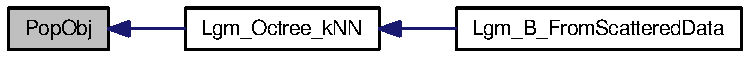
\includegraphics[width=198pt]{_lgm___octree_8h_653f08b2912abb5a5fb6c1761b8a8cec_icgraph}
\end{center}
\end{figure}
\hypertarget{_lgm___octree_8h_885f0695706ada1ee750180afe105958}{
\index{Lgm\_\-Octree.h@{Lgm\_\-Octree.h}!Lgm\_\-Octree\_\-kNN@{Lgm\_\-Octree\_\-kNN}}
\index{Lgm\_\-Octree\_\-kNN@{Lgm\_\-Octree\_\-kNN}!Lgm_Octree.h@{Lgm\_\-Octree.h}}
\subsubsection[{Lgm\_\-Octree\_\-kNN}]{\setlength{\rightskip}{0pt plus 5cm}int Lgm\_\-Octree\_\-kNN ({\bf Lgm\_\-Vector} $\ast$ {\em q}, \/  {\bf Lgm\_\-OctreeCell} $\ast$ {\em Root}, \/  int {\em K}, \/  int $\ast$ {\em Kgot}, \/  double {\em MaxDist2}, \/  {\bf Lgm\_\-OctreeData} $\ast$ {\em kNN})}}
\label{_lgm___octree_8h_885f0695706ada1ee750180afe105958}




Definition at line 474 of file Lgm\_\-Octree.c.

Here is the call graph for this function:\nopagebreak
\begin{figure}[H]
\begin{center}
\leavevmode
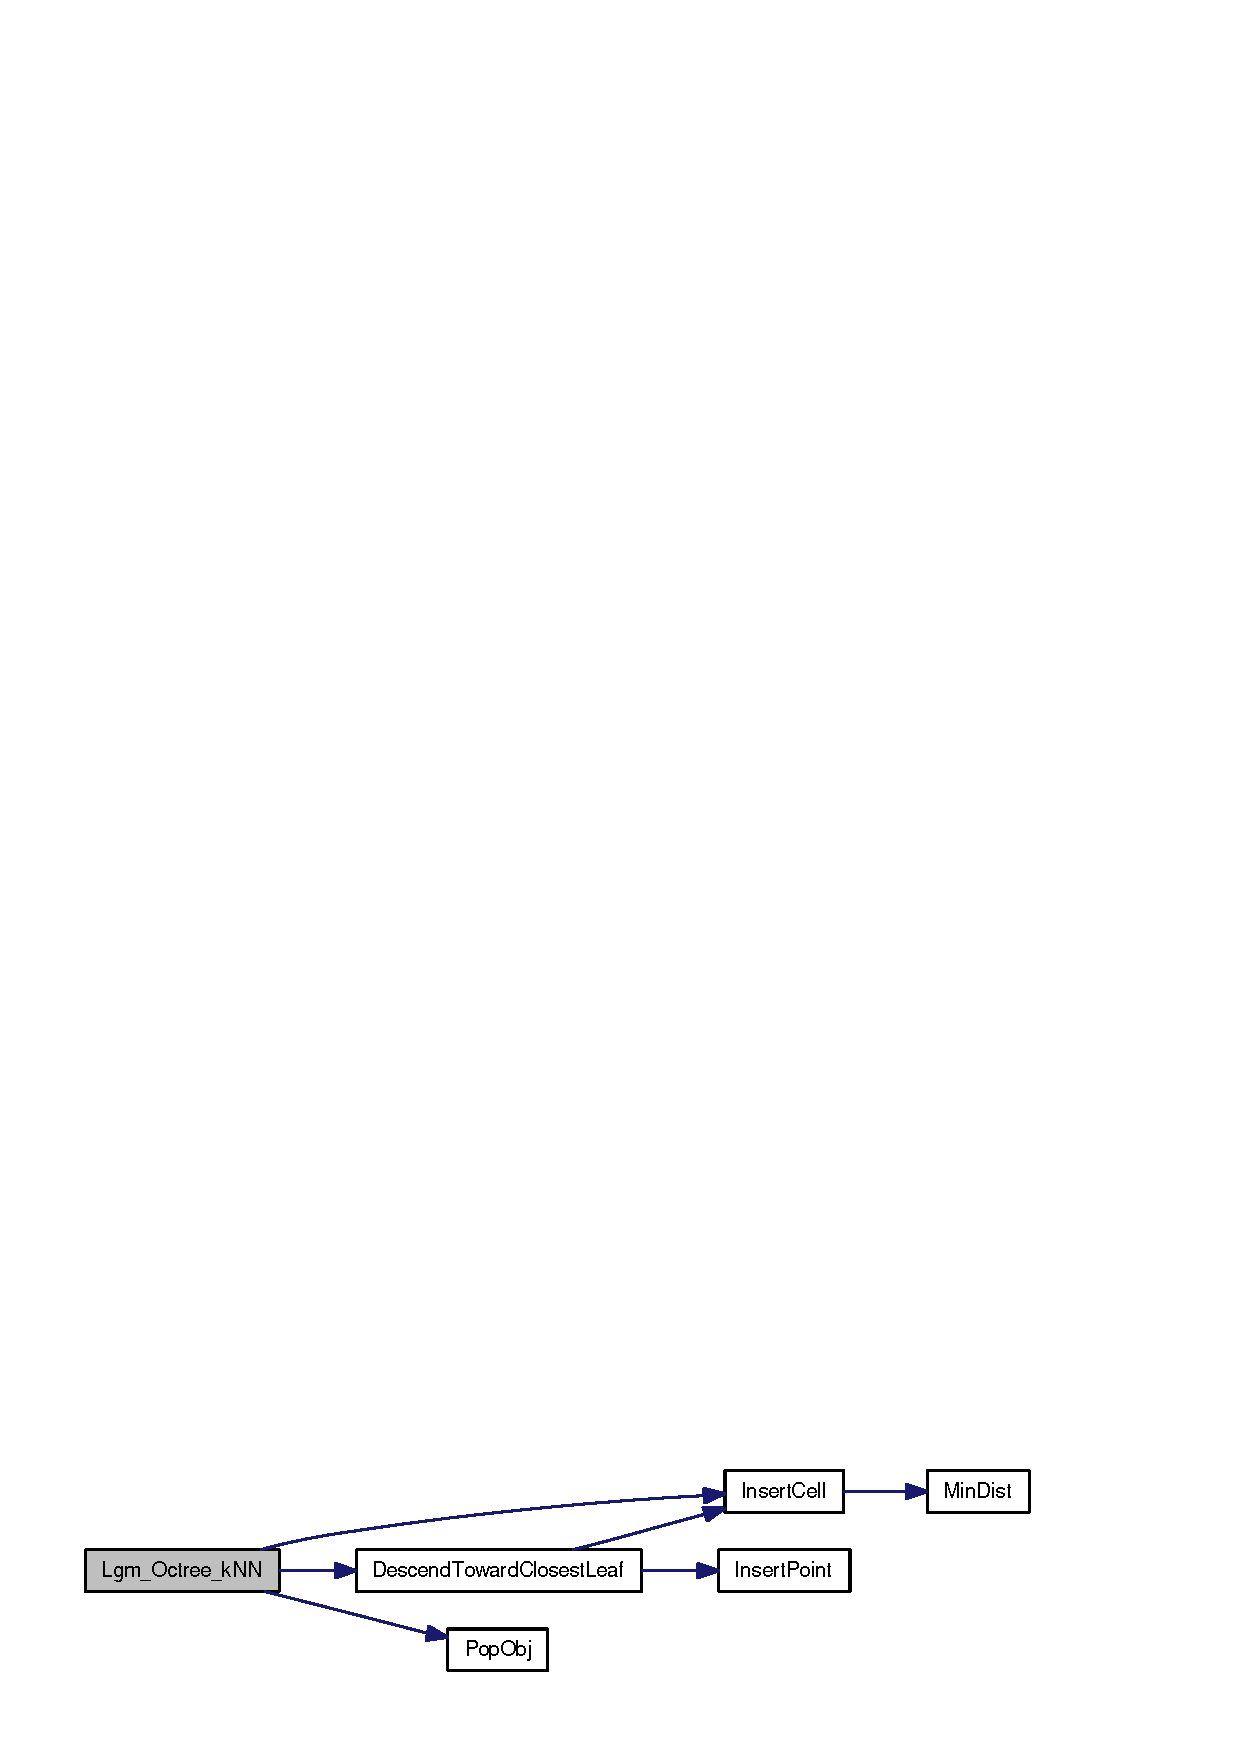
\includegraphics[width=249pt]{_lgm___octree_8h_885f0695706ada1ee750180afe105958_cgraph}
\end{center}
\end{figure}


Here is the caller graph for this function:\nopagebreak
\begin{figure}[H]
\begin{center}
\leavevmode
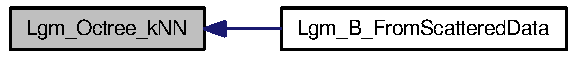
\includegraphics[width=156pt]{_lgm___octree_8h_885f0695706ada1ee750180afe105958_icgraph}
\end{center}
\end{figure}
\hypertarget{_lgm___octree_8h_8faba8ef3514ee1be8aedd369afd4db9}{
\index{Lgm\_\-Octree.h@{Lgm\_\-Octree.h}!CreateNewOctants@{CreateNewOctants}}
\index{CreateNewOctants@{CreateNewOctants}!Lgm_Octree.h@{Lgm\_\-Octree.h}}
\subsubsection[{CreateNewOctants}]{\setlength{\rightskip}{0pt plus 5cm}{\bf Lgm\_\-OctreeCell}$\ast$ CreateNewOctants ({\bf Lgm\_\-OctreeCell} $\ast$ {\em Parent})}}
\label{_lgm___octree_8h_8faba8ef3514ee1be8aedd369afd4db9}




Definition at line 585 of file Lgm\_\-Octree.c.

Here is the caller graph for this function:\nopagebreak
\begin{figure}[H]
\begin{center}
\leavevmode
\includegraphics[width=196pt]{_lgm___octree_8h_8faba8ef3514ee1be8aedd369afd4db9_icgraph}
\end{center}
\end{figure}
\hypertarget{_lgm___octree_8h_3df40f5467250c1b9c2ba1053d38d76f}{
\index{Lgm\_\-Octree.h@{Lgm\_\-Octree.h}!SubDivideVolume@{SubDivideVolume}}
\index{SubDivideVolume@{SubDivideVolume}!Lgm_Octree.h@{Lgm\_\-Octree.h}}
\subsubsection[{SubDivideVolume}]{\setlength{\rightskip}{0pt plus 5cm}void SubDivideVolume ({\bf Lgm\_\-OctreeCell} $\ast$ {\em Vol})}}
\label{_lgm___octree_8h_3df40f5467250c1b9c2ba1053d38d76f}




Definition at line 654 of file Lgm\_\-Octree.c.

Here is the call graph for this function:\nopagebreak
\begin{figure}[H]
\begin{center}
\leavevmode
\includegraphics[width=136pt]{_lgm___octree_8h_3df40f5467250c1b9c2ba1053d38d76f_cgraph}
\end{center}
\end{figure}


Here is the caller graph for this function:\nopagebreak
\begin{figure}[H]
\begin{center}
\leavevmode
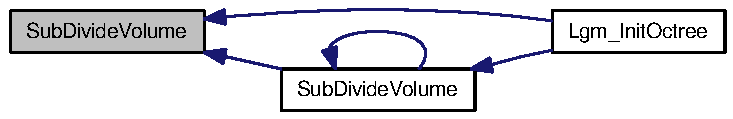
\includegraphics[width=194pt]{_lgm___octree_8h_3df40f5467250c1b9c2ba1053d38d76f_icgraph}
\end{center}
\end{figure}
\hypertarget{_lgm___octree_8h_20080c6b6bf182550e7c1e99d3807020}{
\index{Lgm\_\-Octree.h@{Lgm\_\-Octree.h}!Lgm\_\-InitOctree@{Lgm\_\-InitOctree}}
\index{Lgm\_\-InitOctree@{Lgm\_\-InitOctree}!Lgm_Octree.h@{Lgm\_\-Octree.h}}
\subsubsection[{Lgm\_\-InitOctree}]{\setlength{\rightskip}{0pt plus 5cm}{\bf Lgm\_\-OctreeCell}$\ast$ Lgm\_\-InitOctree ({\bf Lgm\_\-Vector} $\ast$ {\em ObjectPoints}, \/  {\bf Lgm\_\-Vector} $\ast$ {\em ObjectData}, \/  unsigned long int {\em N}, \/  double $\ast$ {\em Min}, \/  double $\ast$ {\em Max}, \/  double $\ast$ {\em Diff})}}
\label{_lgm___octree_8h_20080c6b6bf182550e7c1e99d3807020}




Definition at line 767 of file Lgm\_\-Octree.c.

Here is the call graph for this function:\nopagebreak
\begin{figure}[H]
\begin{center}
\leavevmode
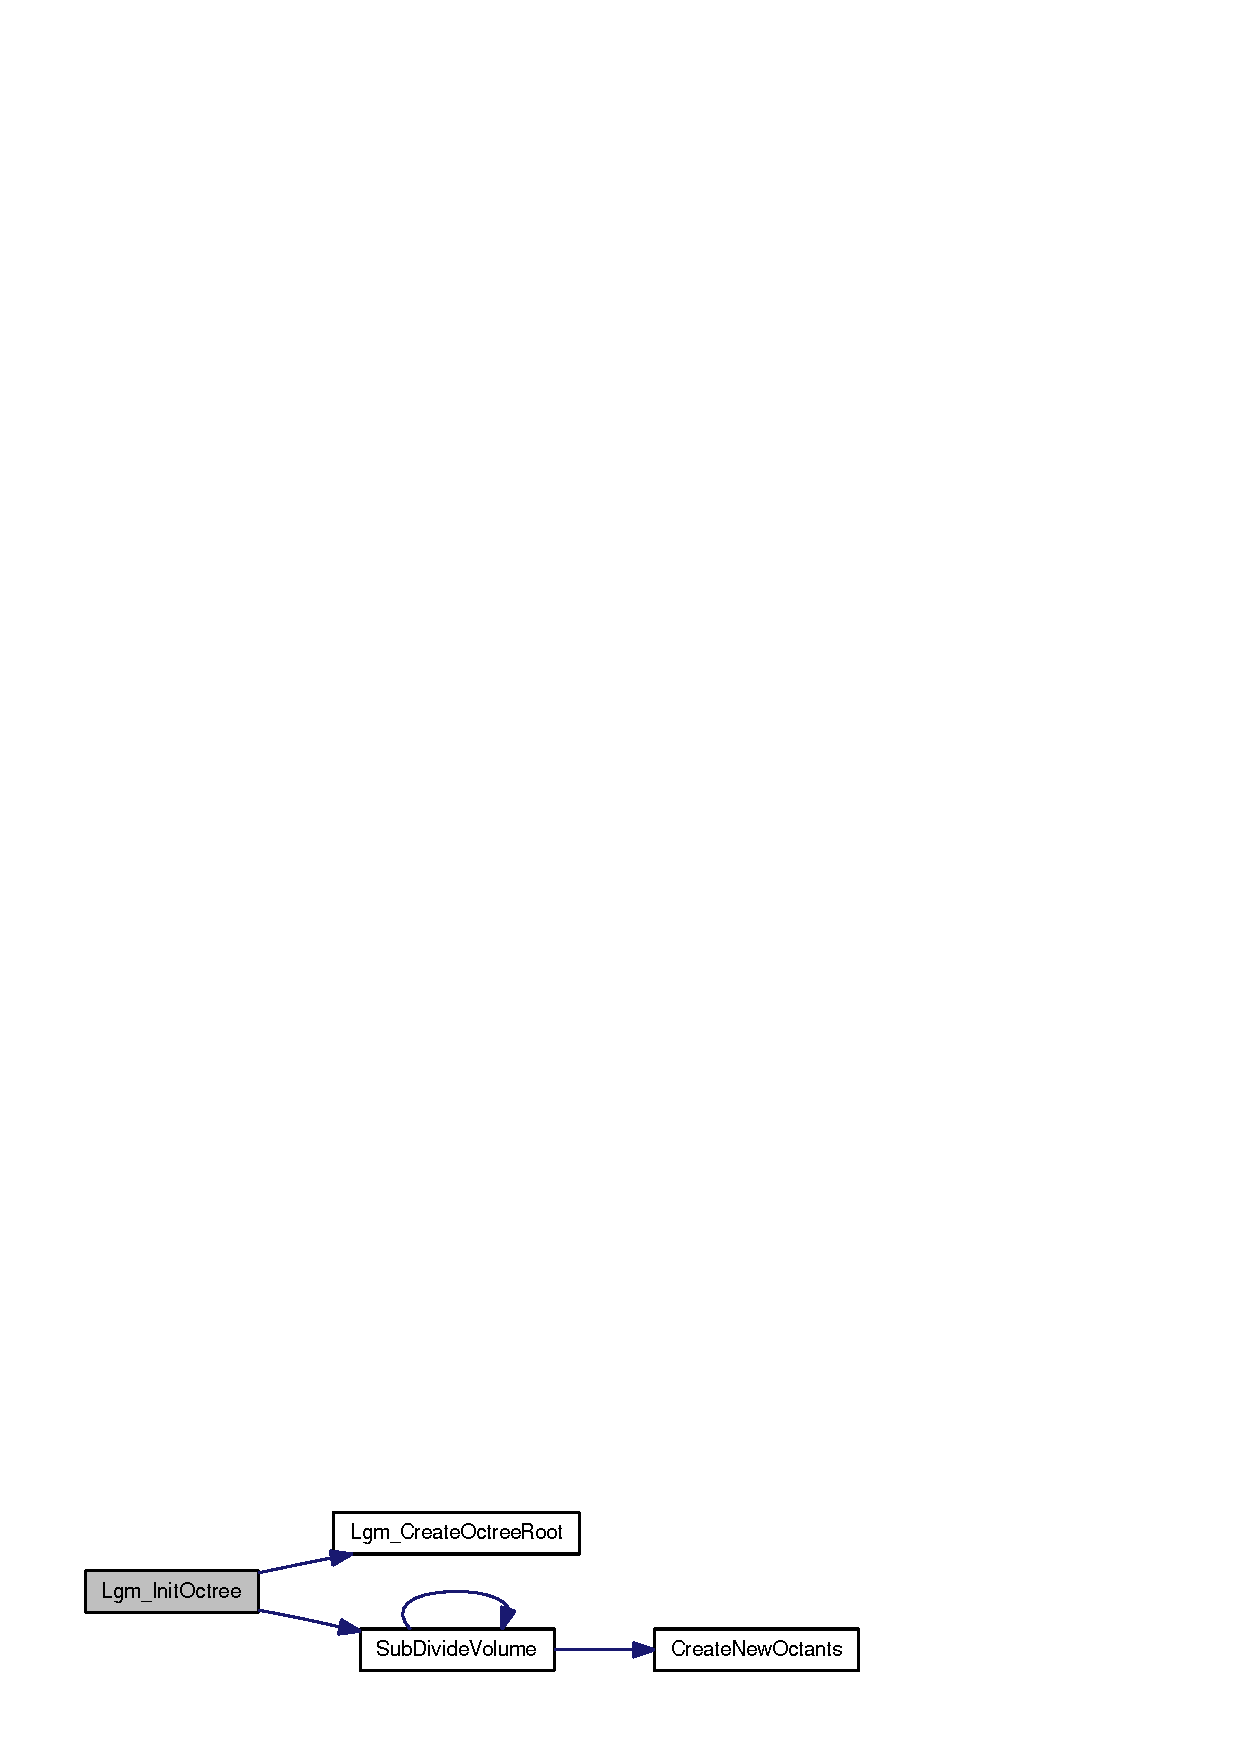
\includegraphics[width=208pt]{_lgm___octree_8h_20080c6b6bf182550e7c1e99d3807020_cgraph}
\end{center}
\end{figure}
